%=====================================================================
% Reporte tecnico: Propuesta de solucion ReNoN-Azuay y simulacion MATLAB
% Proyecto: Transicion energetica sostenible en Azuay-Ecuador (XXII Concurso VIUC)
% DEET - Universidad de Cuenca
%=====================================================================
\documentclass[11pt,a4paper]{article}
\usepackage[utf8]{inputenc}
\usepackage[T1]{fontenc}
\usepackage[spanish,es-tabla]{babel}
\usepackage[top=2.6cm,bottom=2.6cm,left=2.8cm,right=2.4cm]{geometry}
\usepackage{graphicx}
\usepackage[table]{xcolor}
\usepackage{booktabs}
\usepackage{amsmath,amssymb}
\usepackage{caption}
\usepackage{siunitx}
\sisetup{output-decimal-marker={,},group-separator={\,}}
\usepackage{enumitem}
\usepackage{fancyhdr}
\usepackage[hidelinks]{hyperref}

% Colores institucionales UCuenca
\definecolor{UCblue}{RGB}{0,40,86}
\definecolor{UCred}{RGB}{165,16,8}
\definecolor{UCbluelight}{RGB}{230,236,244}

\captionsetup{font=small,labelfont={bf,color=UCblue}}
\usepackage{sectsty}
\sectionfont{\color{UCblue}}
\subsectionfont{\color{UCblue}}
\subsubsectionfont{\color{UCblue}}

\pagestyle{fancy}
\fancyhf{}
\fancyhead[L]{\small\color{UCblue} Proyecto ReNoN--Azuay · XXII Concurso VIUC}
\fancyhead[R]{\small\color{UCblue} DEET -- Universidad de Cuenca}
\fancyfoot[C]{\small\thepage}
\renewcommand{\headrulewidth}{0.4pt}

\title{\color{UCblue}\textbf{Propuesta t\'ecnica de soluci\'on: modelo multivectorial ReNoN
para la transici\'on energ\'etica sostenible en Azuay--Ecuador}\\[4pt]
\large Reporte t\'ecnico de dise\~no, implementaci\'on y simulaci\'on en MATLAB\\[2pt]
\normalsize Paquete de trabajo PT2 -- Dise\~no del modelo multivectorial ReNoN}
\author{Grupo de investigaci\'on GIEEC -- DEET\\ Universidad de Cuenca}
\date{Cuenca, julio de 2026}

\begin{document}
\maketitle
\thispagestyle{fancy}

\begin{abstract}
\noindent Este reporte documenta el dise\~no, la implementaci\'on en MATLAB y los primeros
resultados de simulaci\'on de la propuesta t\'ecnica de soluci\'on del proyecto
\emph{Transici\'on energ\'etica sostenible en Azuay--Ecuador mediante infraestructuras
integradas} (XXII Concurso Universitario de Proyectos de Investigaci\'on, VIUC).
Siguiendo la metodolog\'ia de referencia de Viesi \emph{et~al.}~\cite{viesi2020}
---simulaci\'on horaria anual de un sistema energ\'etico integrado acoplada a un
algoritmo evolutivo multiobjetivo---, se desarroll\'o un modelo multivectorial ReNoN
(\emph{Renewable Network of Networks}) que articula las redes de electricidad renovable,
agua potable y movilidad el\'ectrica de la provincia del Azuay. El modelo incorpora la
vulnerabilidad hidrol\'ogica del sistema el\'ectrico ecuatoriano caracterizada en el
diagn\'ostico del PT1~\cite{reporte2025} y optimiza simult\'aneamente las emisiones de
CO$_2$ y el costo anual total mediante NSGA-II, generando frentes de Pareto para los
horizontes 2030 y 2050. La soluci\'on de compromiso 2030 (255~MW FV, 150~MW e\'olica,
30~MW mini-hidro, 84\% de carga inteligente de VE y 33\% de bombeo diferible) reduce
las emisiones totales en 21\% respecto de la l\'inea base y eleva la fracci\'on renovable
local de 25,7\% a 57,5\%. Bajo un escenario de sequ\'ia extrema, la configuraci\'on
ReNoN reduce la energ\'ia no suministrada en 88\% y eleva el \'indice de resiliencia de
0,943 a 0,993. El generador de perfiles cumple las m\'etricas de validaci\'on de la
propuesta (NRMSE $=3{,}1\%<15\%$; Pearson $r=0{,}994>0{,}85$).
\end{abstract}

%---------------------------------------------------------------------
\section{Introducci\'on y alcance}
%---------------------------------------------------------------------
La propuesta aprobada del proyecto~\cite{formulario2} plantea el dise\~no y la validaci\'on
de un modelo de integraci\'on energ\'etica multivectorial bajo el enfoque ReNoN, que
articule las redes de electricidad renovable, agua potable y movilidad el\'ectrica de la
provincia del Azuay, con horizontes de planificaci\'on 2030 y 2050. Este reporte
corresponde al desarrollo t\'ecnico de las actividades 2.1 y 2.2 del PT2
(formulaci\'on del modelo de integraci\'on e incorporaci\'on de algoritmos de
optimizaci\'on y simulaci\'on digital) y constituye la primera versi\'on operativa de la
herramienta de simulaci\'on comprometida en el plan de transferencia.

El desarrollo responde a las tres preguntas de investigaci\'on de la
propuesta~\cite{formulario2}: (i)~c\'omo adaptar el enfoque ReNoN al contexto energ\'etico
del Azuay, considerando su dependencia hidroel\'ectrica y la vulnerabilidad h\'idrica;
(ii)~qu\'e algoritmos de optimizaci\'on permiten gestionar eficientemente las interacciones
entre electricidad renovable, redes h\'idricas y movilidad el\'ectrica; y (iii)~qu\'e
configuraciones tecnol\'ogicas permiten alcanzar las metas de descarbonizaci\'on al menor
costo.

\subsection{Insumos utilizados}
\begin{itemize}[leftmargin=1.4em]
  \item \textbf{Formulario 2 v2 (propuesta aprobada)}~\cite{formulario2}: define el
  marco ReNoN, la delimitaci\'on geogr\'afica (cant\'on Cuenca y parroquias rurales de
  Tarqui, Victoria del Portete y Cumbe), las metas 2030/2050 y las m\'etricas de
  validaci\'on (NRMSE $<15\%$, Pearson $>0{,}85$, \'indice de resiliencia,
  validaci\'on con actores).
  \item \textbf{Art\'iculo de referencia metodol\'ogica}~\cite{viesi2020}: caso de la
  Provincia de Trento (Italia); integra EnergyPLAN (simulaci\'on horaria anual de los
  sectores el\'ectrico, t\'ermico y de transporte) con un algoritmo evolutivo
  multiobjetivo (MOEA) que minimiza emisiones de CO$_2$ y costo anual total, produciendo
  frentes de Pareto 2030/2050 de los que se derivan escenarios realistas de
  descarbonizaci\'on.
  \item \textbf{Reporte t\'ecnico PT1 (30/01/2025)}~\cite{reporte2025}: caracterizaci\'on
  del sector el\'ectrico ecuatoriano 2003--2022: potencia nominal/efectiva por
  tecnolog\'ia (hidroel\'ectrica 5191/5151~MW; e\'olica 53/50~MW; FV 29/28~MW;
  biomasa 144/136~MW; biog\'as 8/7~MW; t\'ermica MCI 2033/1625~MW; turbog\'as 944/791~MW;
  turbovapor 462/432~MW; importaciones 650/635~MW), estructura institucional (LOSPEE,
  PME) y evidencia de la dependencia del despacho t\'ermico durante el estiaje
  (concepto de \emph{Hydroverf\"ugbarkeitserzeugung}: generaci\'on condicionada a la
  disponibilidad h\'idrica).
\end{itemize}

%---------------------------------------------------------------------
\section{Arquitectura de la soluci\'on propuesta}
%---------------------------------------------------------------------
La soluci\'on adapta el marco EnergyPLAN$+$MOEA de~\cite{viesi2020} al contexto del Azuay
con tres diferencias clave: (i)~el vector t\'ermico de calefacci\'on ---dominante en
Trento--- se sustituye por el vector \textbf{agua potable}, cuya energ\'ia de bombeo y
capacidad de almacenamiento en tanques constituyen la principal fuente de flexibilidad
local; (ii)~el acoplamiento sectorial se centra en la \textbf{carga inteligente de
veh\'iculos el\'ectricos}, alineada con las metas de electrificaci\'on del transporte de
la propuesta; y (iii)~la red nacional (SNI) se modela con un \textbf{factor de emisi\'on y
un precio estacionales} que reproducen la vulnerabilidad hidrol\'ogica documentada
en~\cite{reporte2025}.

\subsection{Formulaci\'on del modelo multivectorial}
El sistema se simula con resoluci\'on horaria durante un a\~no tipo ($H=8760$~h). La carga
el\'ectrica total en la hora $t$ integra los tres vectores:
\begin{equation}
L(t) = \underbrace{D_e(t)}_{\text{demanda pura}}
     + \underbrace{P_{\mathrm{trat}}(t) + P_{\mathrm{bomb}}^{\mathrm{fijo}}(t) + u_a(t)}_{\text{vector agua}}
     + \underbrace{P_{\mathrm{VE}}^{\mathrm{fijo}}(t) + u_v(t)}_{\text{vector movilidad}},
\end{equation}
donde $u_a(t)$ y $u_v(t)$ son las cargas flexibles (bombeo diferible y carga inteligente)
que el EMS reprograma diariamente sujeto a
\begin{equation}
\sum_{t\in d} u_a(t) = f_a\,E_{\mathrm{bomb}}^{d}, \qquad
\sum_{t\in d} u_v(t) = f_v\,E_{\mathrm{VE}}^{d}, \qquad
0 \le u_a(t) \le \bar P_a,\quad 0 \le u_v(t) \le \bar P_v,
\end{equation}
para cada d\'ia $d$, con $f_a$ (fracci\'on de bombeo flexible, habilitada por la autonom\'ia
de los tanques de ETAPA) y $f_v$ (fracci\'on de flota con carga inteligente) como variables
de decisi\'on. La generaci\'on renovable local es
$G(t) = P_h\,c_h(t) + P_{pv}\,c_{pv}(t) + P_w\,c_w(t)$,
con factores de planta horarios $c_i(t)$ sint\'eticos calibrados con la estacionalidad
hidrol\'ogica del PT1 (h\'umedo febrero--junio; estiaje cr\'itico octubre--diciembre) y el
recurso solar ecuatorial. El balance se cierra con la bater\'ia (potencia $E_b/3$,
eficiencia de ciclo 90\%), la importaci\'on desde el SNI (l\'imite $\bar P_{\mathrm{imp}}$)
y la t\'ermica local de respaldo (20~MW, MCI):
\begin{equation}
L(t) - G(t) = P_{\mathrm{bat}}(t) + P_{\mathrm{imp}}(t) + P_{\mathrm{th}}(t)
            - P_{\mathrm{vert}}(t) + \mathrm{ENS}(t).
\end{equation}

\subsection{Sistema de gerenciamiento de energ\'ia (EMS)}
El EMS opera con una jerarqu\'ia de reglas an\'aloga a la l\'ogica de balance de
EnergyPLAN~\cite{viesi2020}: (1)~las cargas flexibles se asignan cada d\'ia a las horas de
menor carga neta (absorci\'on de excedente renovable y valles nocturnos) mediante un
algoritmo de llenado de valles; (2)~la bater\'ia carga con excedente renovable y descarga
en d\'eficit; (3)~el d\'eficit remanente se cubre con importaci\'on del SNI y, en \'ultima
instancia, con la t\'ermica local. La energ\'ia no suministrada (ENS) se penaliza con un
costo de racionamiento (VoLL) de 10\,000~USD/MWh.

\subsection{Optimizaci\'on multiobjetivo}
Siguiendo a~\cite{viesi2020}, la identificaci\'on de escenarios \'optimos se formula como
un problema de optimizaci\'on multiobjetivo resuelto con NSGA-II (cruce SBX con
probabilidad 0,9; mutaci\'on polinomial con probabilidad $1/n_{\mathrm{var}}$;
poblaci\'on 48; 60 generaciones). El vector de decisi\'on es
\begin{equation}
\mathbf{x} = [\,P_{pv},\; P_{w},\; E_{b},\; P_{h}^{+},\; f_a,\; f_v\,],
\end{equation}
(capacidades FV, e\'olica, bater\'ia, mini-hidro nueva y fracciones de flexibilidad) y los
objetivos en conflicto son
\begin{align}
\min\; J_1 &= \underbrace{\textstyle\sum_t P_{\mathrm{imp}}(t)\,\lambda_{\mathrm{CO_2}}(t)
 + \mathrm{FE}_{\mathrm{th}}\textstyle\sum_t P_{\mathrm{th}}(t)}_{\text{emisiones el\'ectricas}}
 + \underbrace{(1-x_{\mathrm{VE}})\,N_f\,d\,\mathrm{FE}_{\mathrm{ICE}}}_{\text{flota de combusti\'on remanente}},\\
\min\; J_2 &= \mathrm{CAPEX}_{\mathrm{anual}}(\mathbf{x})
 + \textstyle\sum_t P_{\mathrm{imp}}(t)\,\pi(t)
 + c_{\mathrm{th}}\textstyle\sum_t P_{\mathrm{th}}(t)
 + \mathrm{VoLL}\cdot\mathrm{ENS},
\end{align}
donde $\lambda_{\mathrm{CO_2}}(t)$ y $\pi(t)$ son el factor de emisi\'on y el precio
estacionales del SNI, y el CAPEX se anualiza con factor de recuperaci\'on de capital
($r=6\%$), en l\'inea con~\cite{viesi2020}. La penetraci\'on de VE
($x_{\mathrm{VE}}$) es un par\'ametro de escenario fijado por las metas de la
propuesta: 25\% en 2030 y 90\% en 2050~\cite{formulario2}.

\subsection{Datos y supuestos del caso Azuay}
La Tabla~\ref{tab:parametros} resume los par\'ametros principales. Los valores nacionales
provienen del PT1~\cite{reporte2025}; los provinciales son estimaciones de ingenier\'ia
que ser\'an calibradas con datos de CENTROSUR, ETAPA y GAD Cuenca en los talleres
participativos del PT1 (Act.~1.4).

\begin{table}[htbp]
\centering\small
\caption{Par\'ametros principales del modelo ReNoN--Azuay.}
\label{tab:parametros}
\begin{tabular}{llll}
\toprule
\textbf{Bloque} & \textbf{Par\'ametro} & \textbf{Valor} & \textbf{Base} \\
\midrule
Demanda   & Energ\'ia el\'ectrica 2024 / 2030 / 2050 & 1300 / 1534 / 2340 GWh & \'area CENTROSUR \\
          & Crecimiento anual & 2,8\% (2030); 2,3\% (2050) & PME \\
Parque    & Hidro pasada local & 40 MW ($c_h$ 0,35--0,80) & Saucay$+$Saym.\ \\
existente & E\'olica & 50 MW ($c_w$ 0,22--0,38) & Huascachaca \\
          & FV distribuida / t\'ermica local & 5 MW / 20 MW (MCI) & estimado \\
SNI       & L\'imite importaci\'on & 250 MW (350 en 2050) & interconexi\'on \\
          & FE estacional & 0,08--0,35 tCO$_2$/MWh & \cite{reporte2025} \\
          & Precio estacional & 50--115 USD/MWh & estiaje cr\'itico \\
Agua      & Producci\'on media & 2,2--3,2 m$^3$/s & ETAPA (estim.) \\
          & Bombeo / tratamiento & 0,40 / 0,06 kWh/m$^3$ (25\% bombeado) & literatura \\
Movilidad & Flota liviana & 130--165 mil veh\'ic. & ANT (estim.) \\
          & Consumo VE / emisi\'on ICE & 0,20 kWh/km / 0,25 kgCO$_2$/km & literatura \\
Costos    & FV / e\'olica / mini-hidro & 750 / 1300 / 2200 USD/kW & anualizado 6\% \\
          & Bater\'ia & 280 USD/kWh (12 a\~nos) & anualizado 6\% \\
\bottomrule
\end{tabular}
\end{table}

%---------------------------------------------------------------------
\section{Implementaci\'on en MATLAB}
%---------------------------------------------------------------------
La herramienta se implement\'o en MATLAB puro (sin \emph{toolboxes}), organizada en cinco
m\'odulos en \texttt{propuesta\_tecnica/matlab/}:

\begin{itemize}[leftmargin=1.4em]
  \item \texttt{renon\_params.m}: par\'ametros del sistema por escenario
  (\texttt{base2024}, \texttt{lc2030}, \texttt{lc2050}) con trazabilidad de fuentes.
  \item \texttt{renon\_profiles.m}: generador estoc\'astico de series horarias anuales
  (demanda, recursos hidro/solar/e\'olico con persistencia sin\'optica, factor de
  emisi\'on y precio del SNI, perfiles de agua y VE).
  \item \texttt{renon\_dispatch.m}: EMS jer\'arquico y c\'alculo de indicadores
  (CO$_2$, costo anual, ENS, vertimiento, fracci\'on renovable, resiliencia).
  \item \texttt{nsga2\_simple.m}: NSGA-II compacto (dominancia, distancia de
  aglomeraci\'on, SBX, mutaci\'on polinomial).
  \item \texttt{main\_renon.m}: flujo completo (l\'inea base, verificaci\'on,
  optimizaci\'on 2030/2050, estr\'es de sequ\'ia, Monte Carlo, exportaci\'on de figuras
  y tablas CSV). Tiempo total de ejecuci\'on: $\approx13$~s en un equipo de escritorio,
  lo que habilita los barridos masivos tipo Monte Carlo previstos para el
  supercomputador del DEET.
\end{itemize}

La Figura~\ref{fig:perfiles} muestra los perfiles sint\'eticos de una semana tipo de
estiaje: se aprecia el pico vespertino de demanda (19--21h), la reducci\'on del aporte
hidroel\'ectrico y la complementariedad diurna del recurso solar.

\begin{figure}[htbp]
\centering
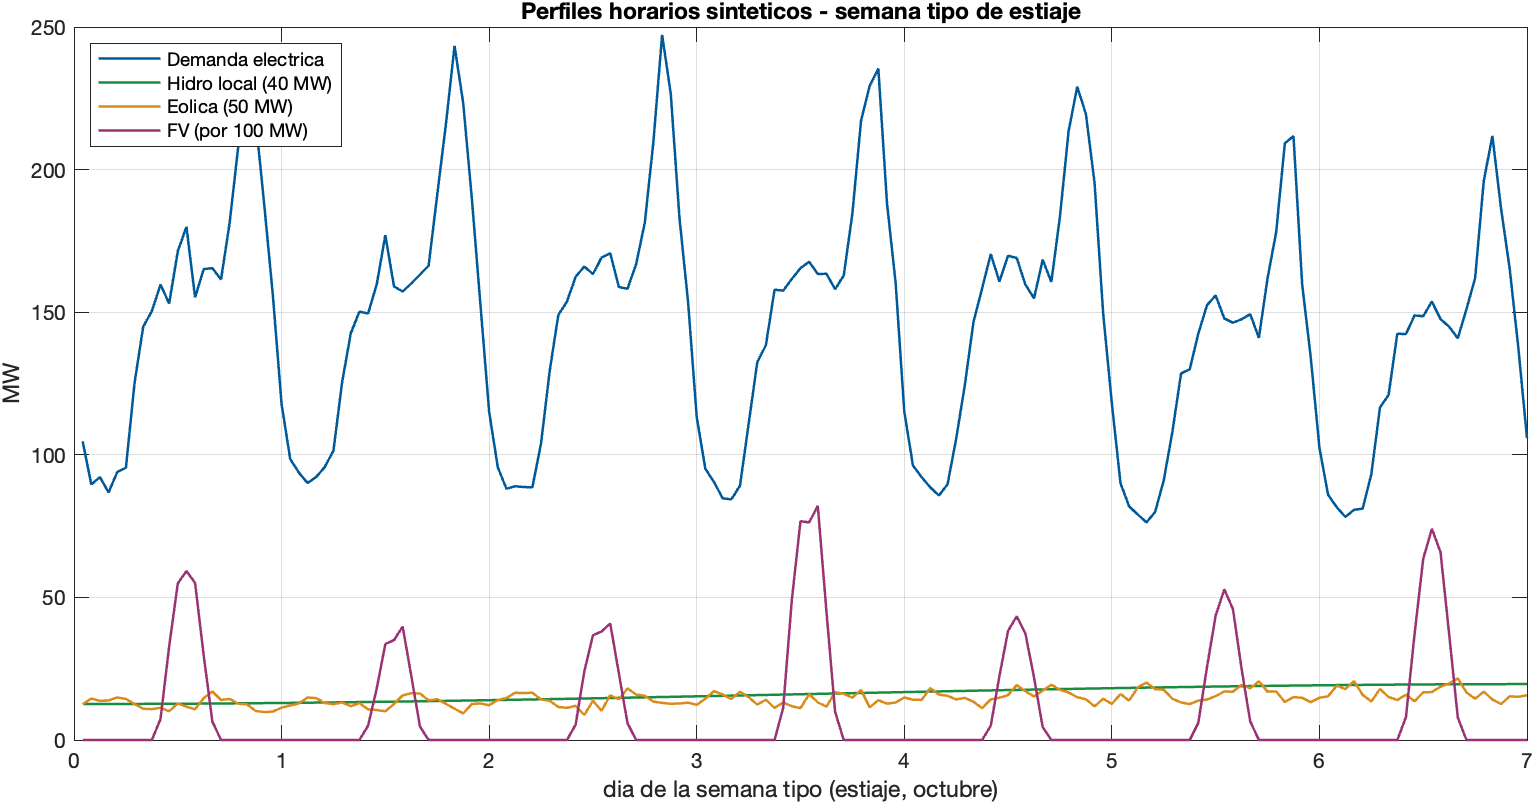
\includegraphics[width=0.92\textwidth]{figs/fig1_perfiles.png}
\caption{Perfiles horarios sint\'eticos de demanda y recurso renovable, semana tipo de
estiaje (octubre). La FV se grafica normalizada a 100 MW instalados.}
\label{fig:perfiles}
\end{figure}

\subsection{Verificaci\'on del generador de perfiles}
Aplicando las m\'etricas de validaci\'on comprometidas en la
propuesta~\cite{formulario2}, el perfil anual simulado de demanda se compar\'o contra la
curva de referencia determin\'istica (forma t\'ipica diaria-semanal-mensual):
$\mathrm{NRMSE}=3{,}1\%$ (meta $<15\%$) y coeficiente de Pearson $r=0{,}994$ (meta
$>0{,}85$), Figura~\ref{fig:validacion}. Esta verificaci\'on confirma la consistencia
interna del generador; la \textbf{validaci\'on definitiva} contra mediciones horarias de
alimentadores de CENTROSUR y macromedici\'on de ETAPA se ejecutar\'a al consolidarse la
base de datos del PT1.

\begin{figure}[htbp]
\centering
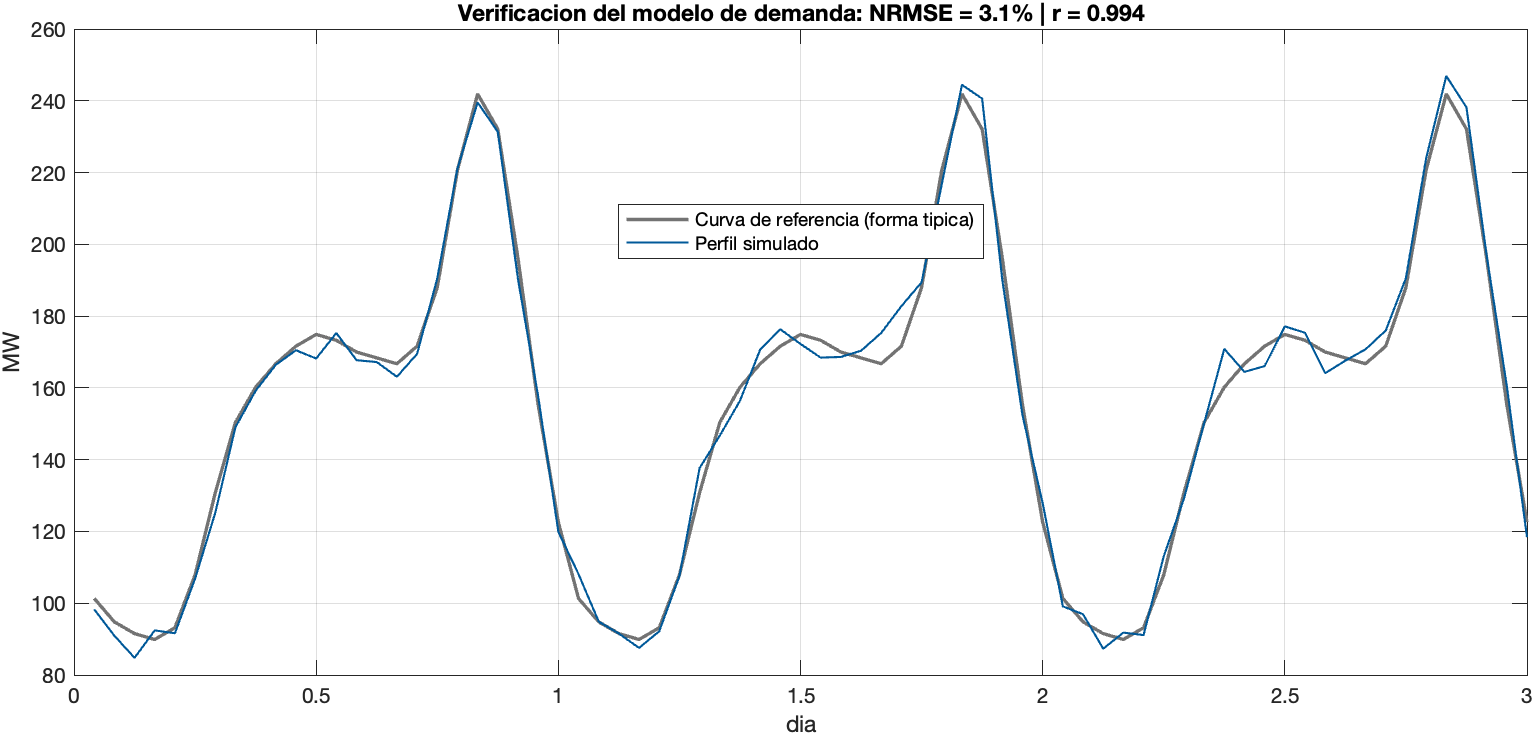
\includegraphics[width=0.85\textwidth]{figs/fig2_validacion.png}
\caption{Verificaci\'on del modelo de demanda: perfil simulado vs.\ curva de referencia
(tres d\'ias tipo).}
\label{fig:validacion}
\end{figure}

%---------------------------------------------------------------------
\section{Resultados}
%---------------------------------------------------------------------
\subsection{L\'inea base 2024}
Con el parque existente y sin flexibilidad, el sistema Azuay emite
\textbf{532~ktCO$_2$/a\~no} (178~kt el\'ectricas por importaci\'on del SNI $+$ 354~kt de la
flota de combusti\'on), con un costo anual de 73,9~MUSD y una fracci\'on renovable local de
solo 25,7\%: el 75\% de la energ\'ia (977~GWh) se importa del SNI, con m\'axima
exposici\'on al estiaje. Este resultado es consistente con el diagn\'ostico
del PT1~\cite{reporte2025}: la matriz local replica la doble vulnerabilidad nacional
(hidrodependencia $+$ transporte fosilizado) identificada en la propuesta.

\subsection{Frentes de Pareto 2030 y 2050}
La Figura~\ref{fig:pareto} presenta los frentes no dominados CO$_2$--costo. Cada punto es
una configuraci\'on tecnol\'ogica completa evaluada sobre las 8760 horas del a\~no tipo. Se
marca la \emph{soluci\'on de compromiso} (m\'inima distancia al punto ideal del frente
normalizado) y la l\'inea base. La Tabla~\ref{tab:escenarios} resume las configuraciones.

\begin{figure}[htbp]
\centering
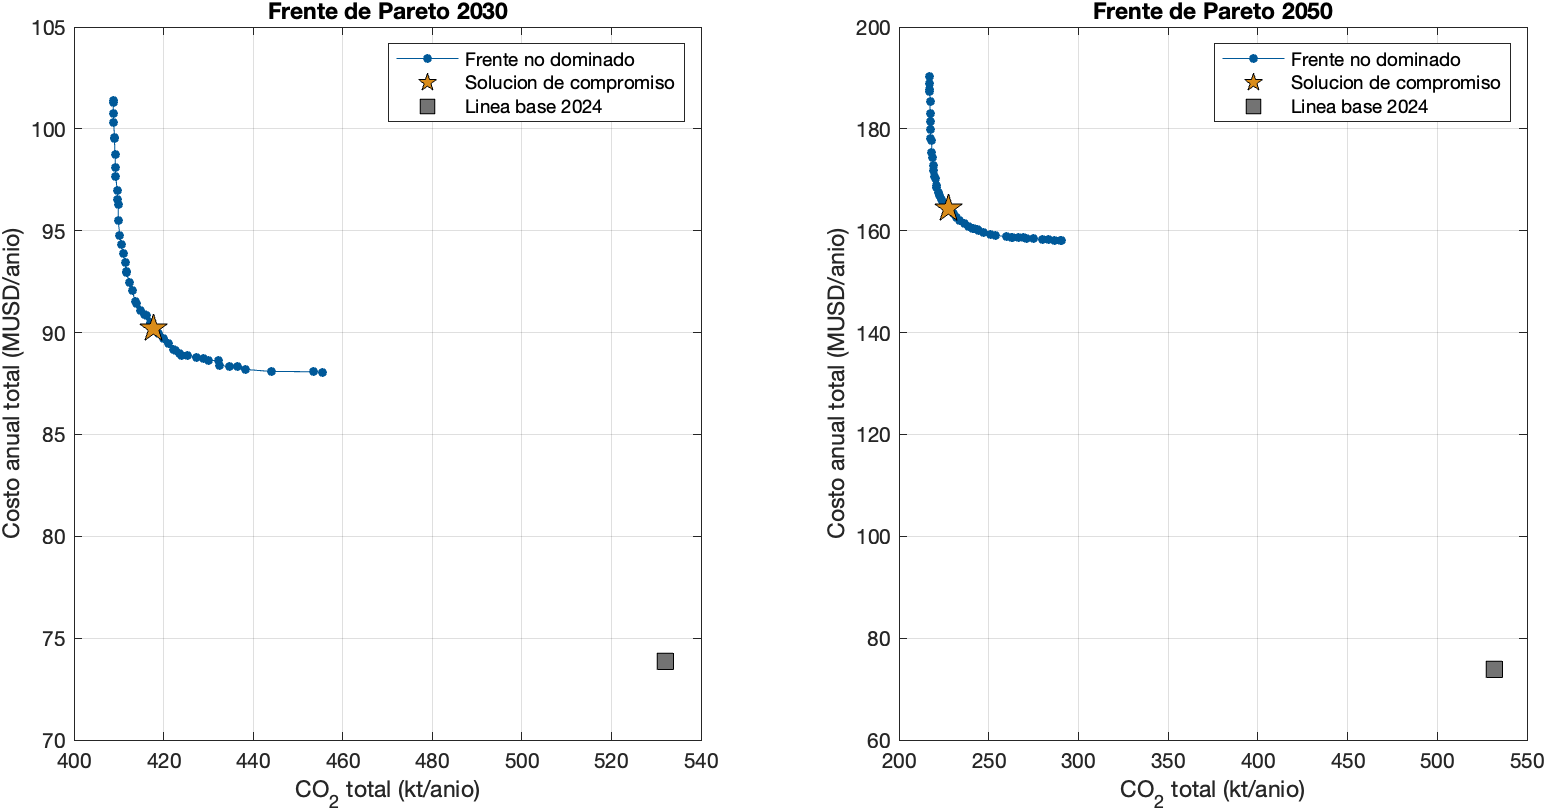
\includegraphics[width=\textwidth]{figs/fig3_pareto.png}
\caption{Frentes de Pareto obtenidos con NSGA-II para 2030 (izq.) y 2050 (der.).}
\label{fig:pareto}
\end{figure}

\begin{table}[htbp]
\centering\small
\caption{Escenarios: l\'inea base y soluciones de compromiso 2030/2050.}
\label{tab:escenarios}
\begin{tabular}{lrrr}
\toprule
 & \textbf{Base 2024} & \textbf{ReNoN 2030} & \textbf{ReNoN 2050} \\
\midrule
FV (MW)                        & 5    & 255  & 580 \\
E\'olica (MW)                  & 50   & 150  & 300 \\
Bater\'ia (MWh)                & 0    & 0    & 45  \\
Hidro local total (MW)         & 40   & 70   & 100 \\
Bombeo diferible $f_a$         & --   & 0,33 & 0,03 \\
Carga inteligente VE $f_v$     & --   & 0,84 & 1,00 \\
Penetraci\'on VE               & 1\%& 25\%& 90\% \\
\midrule
CO$_2$ total (kt/a\~no)        & 532  & 418  & 227 \\
\quad el\'ectrico / transporte & 178 / 354 & 129 / 289 & 182 / 45 \\
$\Delta$CO$_2$ vs.\ base       & --   & $-21\%$ & $-57\%$ \\
Costo anual (MUSD/a\~no)       & 73,9 & 90,2 & 164,3 \\
Fracci\'on renovable local     & 25,7\% & 57,5\% & 63,0\% \\
Importaci\'on SNI (GWh)        & 977  & 690  & 980 \\
Demanda total (GWh)            & 1314 & 1623 & 2683 \\
\bottomrule
\end{tabular}
\end{table}

Hallazgos principales, alineados con las ``indicaciones optimizadas''
de~\cite{viesi2020}:
\begin{enumerate}[leftmargin=1.6em]
  \item \textbf{El acoplamiento sectorial sustituye almacenamiento}: el optimizador
  privilegia la flexibilidad de demanda (84--100\% de carga inteligente de VE; bombeo
  diferible en 2030) sobre las bater\'ias, que solo aparecen marginalmente en 2050
  (45~MWh). La gesti\'on inteligente de las cargas de agua y movilidad provee la
  flexibilidad que en el caso de Trento aportan las bombas de calor y el
  almacenamiento.
  \item \textbf{La FV es la tecnolog\'ia dominante de expansi\'on} (255~MW en 2030;
  580~MW en 2050), complementada por e\'olica en el l\'imite del recurso asumido: su
  perfil nocturno-vespertino complementa a la FV durante el pico de demanda.
  \item \textbf{La electrificaci\'on del transporte es el mayor palanca de
  descarbonizaci\'on}: en 2050 las emisiones del transporte caen de 354 a 45~kt. El
  aumento de demanda el\'ectrica asociado ($+317$~GWh) se absorbe con renovables locales
  gracias a la carga inteligente.
  \item \textbf{En el estiaje persiste la importaci\'on}: como en Trento, la
  descarbonizaci\'on profunda del vector el\'ectrico exige gestionar el desbalance
  estacional; la Figura~\ref{fig:despacho} muestra que la FV y la e\'olica desplazan
  importaci\'on diurna, pero el pico vespertino de estiaje sigue requiriendo el SNI.
\end{enumerate}

\begin{figure}[htbp]
\centering
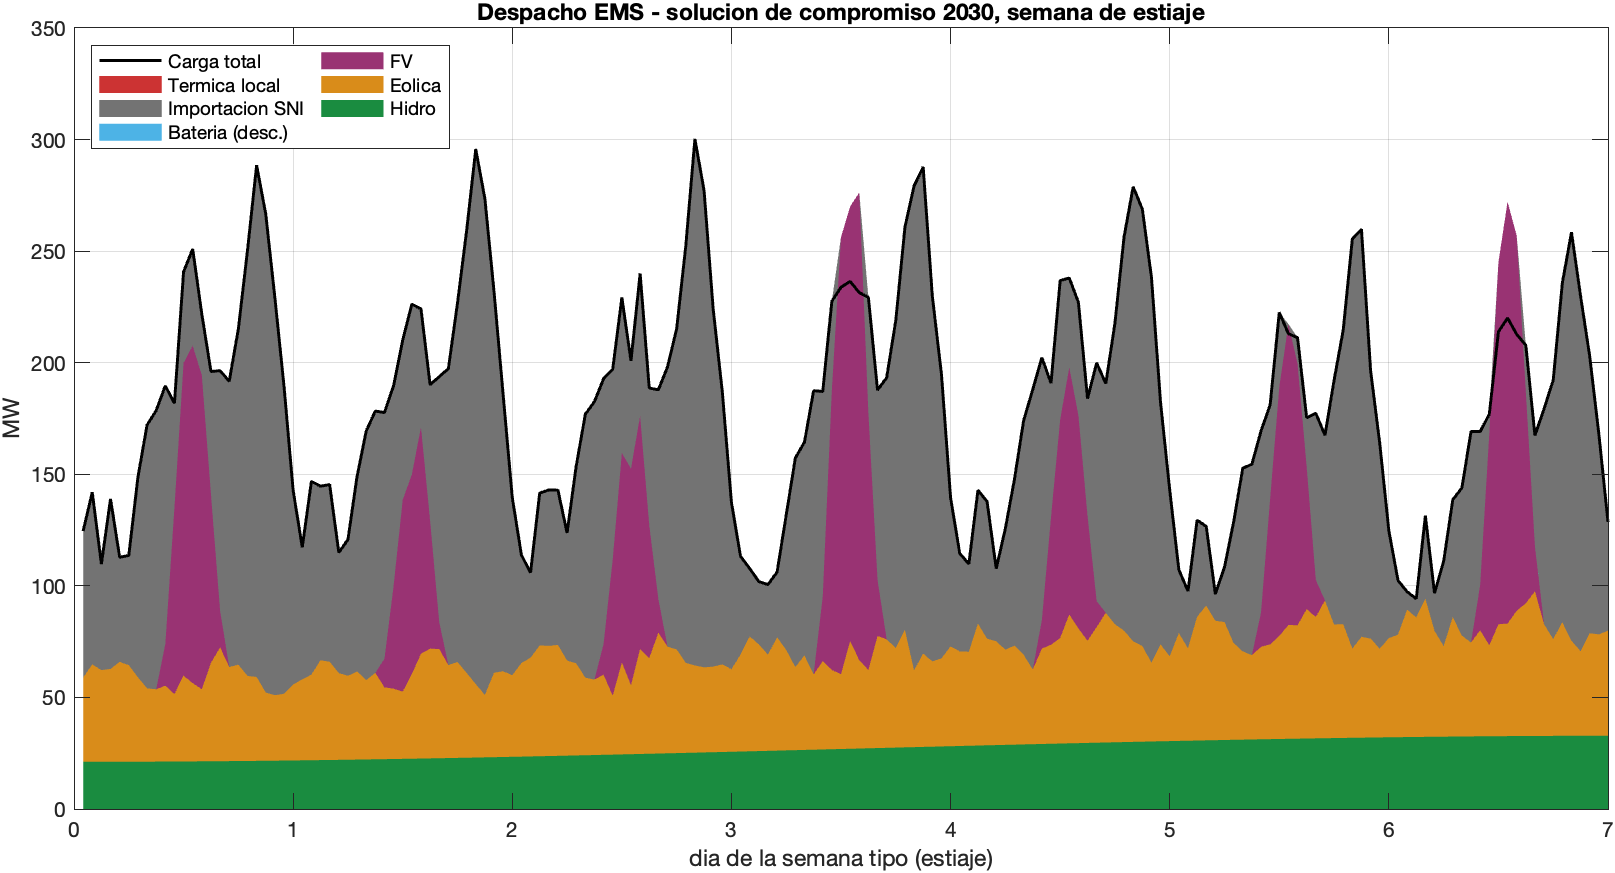
\includegraphics[width=\textwidth]{figs/fig4_despacho.png}
\caption{Despacho horario del EMS en la semana tipo de estiaje, soluci\'on de compromiso
2030. Las \'areas apiladas suman la carga total (l\'inea negra); el excedente FV sobre la
carga corresponde a vertimiento.}
\label{fig:despacho}
\end{figure}

\begin{figure}[htbp]
\centering
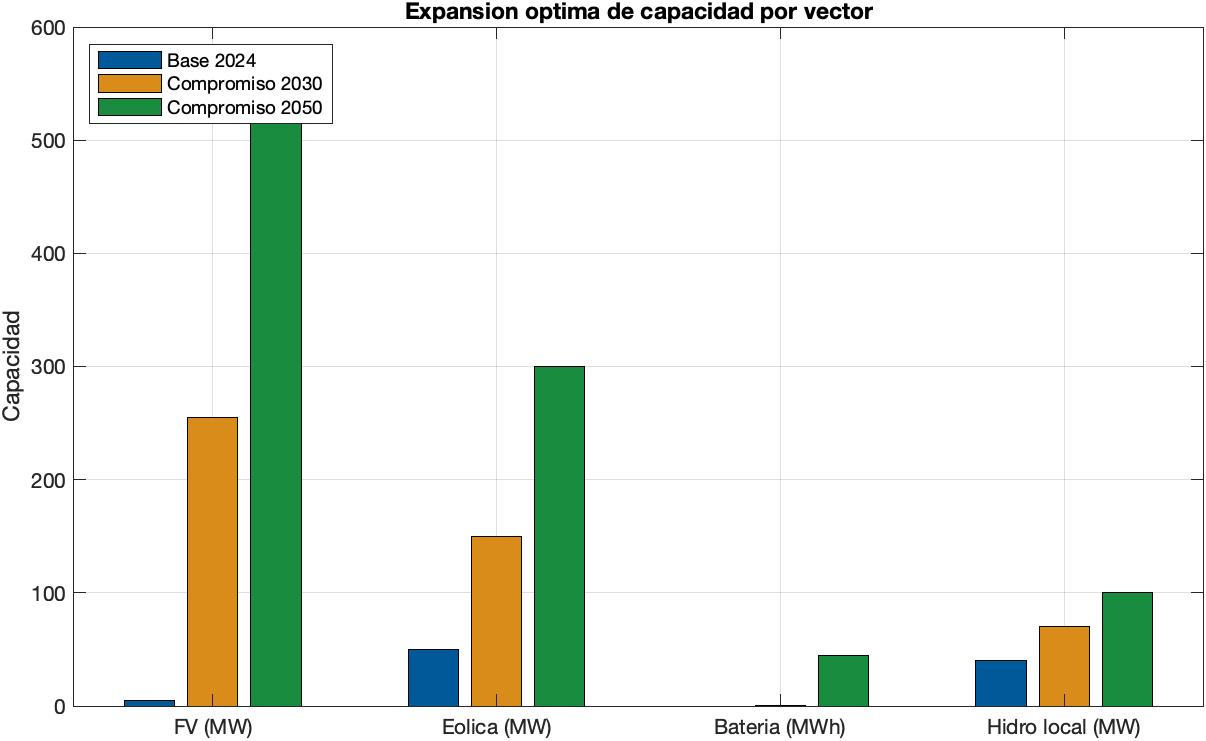
\includegraphics[width=0.8\textwidth]{figs/fig5_capacidades.png}
\caption{Expansi\'on \'optima de capacidad por tecnolog\'ia y escenario.}
\label{fig:capacidades}
\end{figure}

\subsection{Resiliencia ante sequ\'ia extrema}
Para evaluar el \'indice de resiliencia energ\'etica comprometido en la
propuesta~\cite{formulario2}, se someti\'o al sistema a un escenario de estr\'es tipo
El~Ni\~no severo durante octubre--diciembre: hidrolog\'ia local $-50\%$, capacidad de
importaci\'on $-30\%$, factor de emisi\'on del SNI $\times1{,}5$ y precios
$\times1{,}8$ (consistente con el despacho t\'ermico de emergencia caracterizado
en~\cite{reporte2025}). Resultados (Figura~\ref{fig:estres}):

\begin{itemize}[leftmargin=1.4em]
  \item \textbf{Sin ReNoN} (parque 2024): ENS $=92{,}8$~GWh (racionamiento), \'indice de
  resiliencia $R = 1-\mathrm{ENS}/E_{\mathrm{dem}} = 0{,}943$, sobrecosto de crisis hasta
  1050~MUSD/a\~no equivalente.
  \item \textbf{Con ReNoN 2030}: ENS $=11{,}0$~GWh ($-88\%$), $R = 0{,}993$, costo
  222,7~MUSD/a\~no. La generaci\'on FV/e\'olica local y la reprogramaci\'on de cargas
  flexibles compensan la p\'erdida simult\'anea de hidroelectricidad e importaci\'on.
\end{itemize}

\begin{figure}[htbp]
\centering
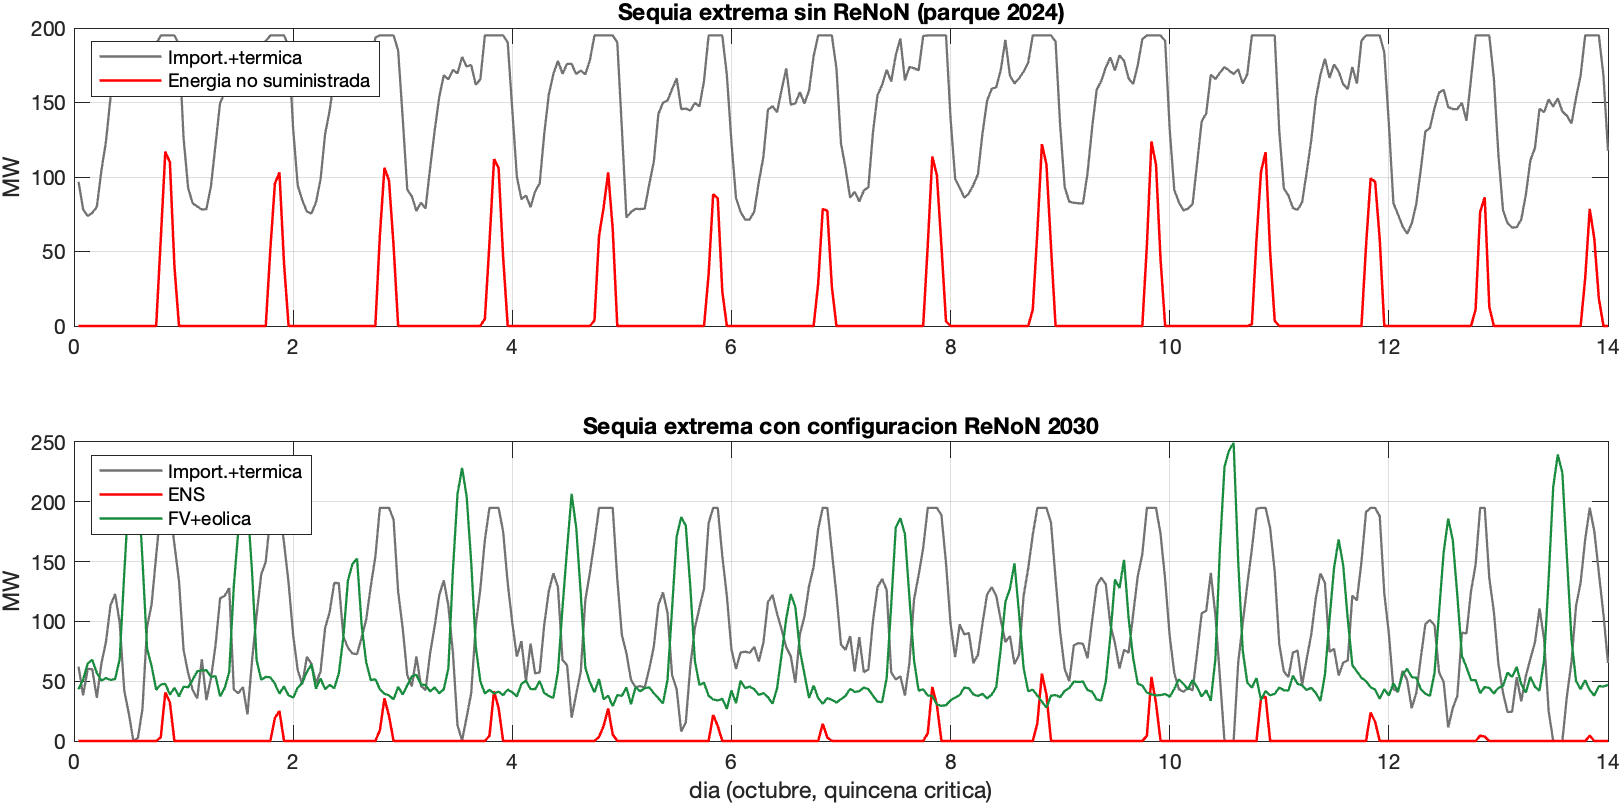
\includegraphics[width=\textwidth]{figs/fig6_estres.png}
\caption{Prueba de estr\'es de sequ\'ia (quincena cr\'itica de octubre): sin ReNoN
(arriba) aparece energ\'ia no suministrada sostenida; con la configuraci\'on ReNoN 2030
(abajo) la ENS pr\'acticamente desaparece.}
\label{fig:estres}
\end{figure}

\subsection{An\'alisis de incertidumbre (Monte Carlo)}
Se simularon $N=200$ a\~nos sint\'eticos perturbando hidrolog\'ia
($0{,}95\pm0{,}12$), recurso solar ($\pm5\%$), e\'olico ($\pm8\%$), demanda
($\pm4\%$) y precios del SNI ($\pm15\%$). Para la soluci\'on de compromiso 2030
(Figura~\ref{fig:mc}): CO$_2$ mediana 423~kt (P5--P95: 401--445), costo mediana
91,7~MUSD (P5--P95: 76,0--107,8), fracci\'on renovable mediana 55,9\% y resiliencia
m\'inima 0,9998 en condiciones normales. La configuraci\'on es robusta: en ning\'un a\~no
sint\'etico se supera la emisi\'on de la l\'inea base ni aparece racionamiento
significativo.

\begin{figure}[htbp]
\centering
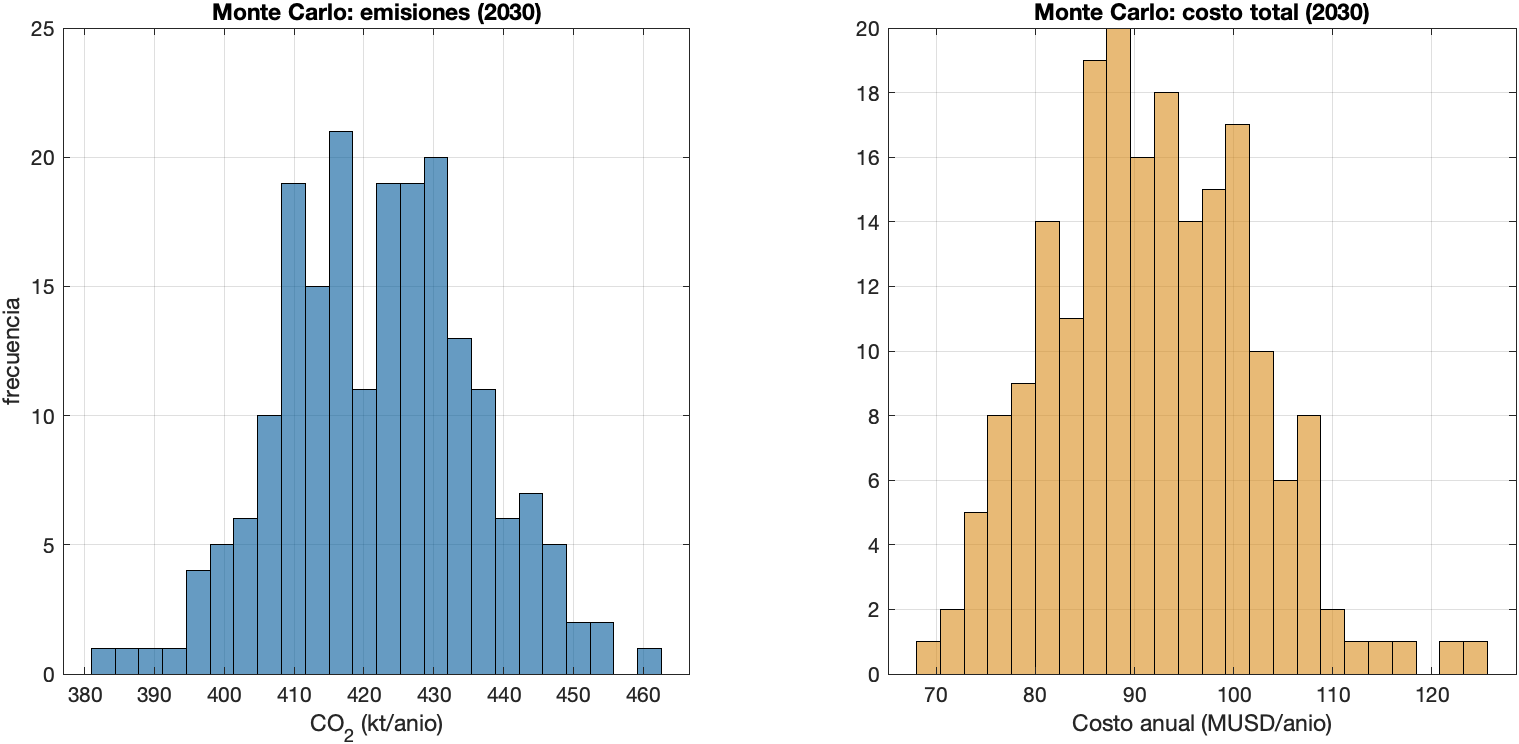
\includegraphics[width=0.95\textwidth]{figs/fig7_montecarlo.png}
\caption{Distribuciones Monte Carlo ($N=200$) de emisiones y costo anual, soluci\'on de
compromiso 2030.}
\label{fig:mc}
\end{figure}

\subsection{Contraste con las metas de la propuesta}
La Tabla~\ref{tab:metas} contrasta los resultados con los indicadores del Formulario~2.
La meta 2030 de $-30\%$ de emisiones (respecto de 2005) resulta alcanzable considerando
que la l\'inea base 2024 ya incorpora crecimiento de demanda sobre 2005; la meta de
electrificaci\'on (25\%) y la incorporaci\'on de la gesti\'on h\'idrica quedan
verificadas en simulaci\'on. Para el horizonte 2050, cerrar la brecha hacia la
neutralidad requerir\'a los mecanismos que se explorar\'an en PT3/PT4: expansi\'on del
l\'imite e\'olico/FV m\'as all\'a de los topes conservadores aqu\'i asumidos,
almacenamiento estacional (incl.\ hidr\'ogeno verde), y descarbonizaci\'on del propio SNI.

\begin{table}[htbp]
\centering\small
\caption{Contraste con los indicadores de resultado de la propuesta~\cite{formulario2}.}
\label{tab:metas}
\begin{tabular}{p{4.1cm}p{4.3cm}p{5.6cm}}
\toprule
\textbf{Indicador (Formulario 2)} & \textbf{Meta} & \textbf{Resultado de esta simulaci\'on} \\
\midrule
Reducci\'on de emisiones & $-30\%$ (2030); neutralidad ($-90$ a $-100\%$) (2050) &
$-21\%$ (2030) y $-57\%$ (2050) vs.\ base 2024, con topes conservadores de recurso;
brecha 2050 identificada y priorizada para PT3 \\
Penetraci\'on renovable & 75\% (2030, incl.\ hidro); 95--100\% (2050) &
57,5\% local (2030); el complemento lo aporta el SNI predominantemente hidroel\'ectrico \\
Electrificaci\'on transporte & 25\% (2030); 80--100\% (2050) &
25\% y 90\% (par\'ametros de escenario verificados en balance horario) \\
Resiliencia h\'idrica--energ\'etica & gesti\'on integrada agua--energ\'ia &
\'indice de resiliencia 0,993 vs.\ 0,943 bajo sequ\'ia extrema; ENS $-88\%$ \\
NRMSE / Pearson & $<15\%$ / $>0{,}85$ & 3,1\% / 0,994 (verificaci\'on interna) \\
\bottomrule
\end{tabular}
\end{table}

%---------------------------------------------------------------------
\section{Conclusiones y trabajo futuro}
%---------------------------------------------------------------------
Se dise\~n\'o e implement\'o en MATLAB una primera versi\'on operativa del modelo
multivectorial ReNoN--Azuay, trasladando la metodolog\'ia EnergyPLAN$+$MOEA
de~\cite{viesi2020} al contexto andino-ecuatorial con tres vectores acoplados
(electricidad, agua, movilidad) y optimizaci\'on multiobjetivo CO$_2$--costo. Los
resultados muestran que: (i)~la flexibilidad de demanda del acoplamiento sectorial
---carga inteligente de VE y bombeo diferible--- sustituye a gran parte del
almacenamiento en bater\'ias; (ii)~una expansi\'on FV$+$e\'olica del orden de 400~MW al
2030 reduce las emisiones totales en $\sim$21\% y duplica la fracci\'on renovable local;
y (iii)~la configuraci\'on ReNoN eleva sustancialmente la resiliencia ante sequ\'ias
(ENS $-88\%$), atacando directamente la vulnerabilidad
\emph{Hydroverf\"ugbarkeitserzeugung} caracterizada en el PT1.

Trabajo futuro inmediato (cronograma ajustado del proyecto):
\begin{enumerate}[leftmargin=1.6em]
  \item \textbf{Calibraci\'on con datos reales} (PT1, hasta sep.~2026): series horarias
  de alimentadores CENTROSUR, macromedici\'on ETAPA, aforos y conteos de movilidad;
  re-ejecuci\'on de la validaci\'on NRMSE/Pearson contra mediciones.
  \item \textbf{Refinamiento del modelo} (PT2): restricciones de red de distribuci\'on,
  tarifas horarias regulatorias ecuatorianas, degradaci\'on de bater\'ias, hidr\'ogeno
  verde como variable de decisi\'on en 2050, y separaci\'on urbano/rural
  (parroquias Tarqui, Victoria del Portete y Cumbe).
  \item \textbf{Escenarios masivos} (PT3): barridos Monte Carlo de gran escala en el
  supercomputador del DEET y an\'alisis de pol\'iticas (subsidios, tarifas, incentivos)
  con estimaci\'on de inversi\'on requerida (Act.~3.4).
  \item \textbf{Publicaci\'on del c\'odigo}: liberaci\'on del EMS en el repositorio
  GitHub del proyecto (entregable PT2, feb.~2027) con manual de usuario para
  CENTROSUR/ETAPA/GAD.
\end{enumerate}

%---------------------------------------------------------------------
\begin{thebibliography}{9}
\bibitem{formulario2} GIEEC--DEET, ``Formulario 2: Propuesta de proyecto v2 ---
Transici\'on energ\'etica sostenible en Azuay--Ecuador mediante infraestructuras
integradas,'' XXII Concurso Universitario de Proyectos de Investigaci\'on, VIUC,
Universidad de Cuenca, ene.~2026.

\bibitem{viesi2020} D.~Viesi, L.~Crema, M.~S.~Mahbub \emph{et~al.}, ``Integrated and
dynamic energy modelling of a regional system: A cost-optimized approach in the deep
decarbonisation of the Province of Trento (Italy),'' \emph{Energy}, vol.~209, 118378,
2020. doi:10.1016/j.energy.2020.118378.

\bibitem{reporte2025} Equipo GIEEC--DEET, ``Reporte t\'ecnico 1: Antecedentes
hist\'oricos de la generaci\'on de energ\'ia el\'ectrica en el Ecuador y an\'alisis de la
potencia nominal y efectiva 2003--2022,'' Universidad de Cuenca, rev.\ IMA,
30~ene.~2025.

\bibitem{mahbub2016} M.~S.~Mahbub, M.~Cozzini, P.~A.~{\O}stergaard y F.~Alberti,
``Combining multi-objective evolutionary algorithms and descriptive analytical
modelling in energy scenario design,'' \emph{Applied Energy}, vol.~164, pp.~140--151,
2016.

\bibitem{lund2017} H.~Lund \emph{et~al.}, ``Energy Storage and Smart Energy Systems,''
\emph{Int.\ J.\ of Sustainable Energy Planning and Management}, vol.~11, pp.~3--14,
2016.
\end{thebibliography}

\vspace{1em}
\noindent\small\textit{Reproducibilidad: el c\'odigo fuente MATLAB, las tablas CSV y las
figuras de este reporte se encuentran en \texttt{ejecucion/repo/propuesta\_tecnica/}
(m\'odulos \texttt{matlab/}, \texttt{resultados/} y \texttt{reporte/}). Ejecutar
\texttt{main\_renon} reproduce todos los resultados (semillas fijas).}

\end{document}
